\chapter{Das Deep Learning Modell}
\section{Analyse der Technologie}
\textit{TensorFlow} ist eine Bibliothek, mit der Deep Learning durchgeführt werden können, es wurde im Jahr 2015 von Google Open Source gemacht. Mit TensorFlow werden die Datan als Tensoren dargestellt und fließen durch Schichten. Dieses ermöglicht die Inferent und das Traiing in maschinellen Lernmodellen. Ein Tensor ist ein multidimensionales Array. In neuronalen Netzen und beim Deep Learning wird jedes Datenelement und jedes Berechnungsergebnis als Tensor dargestellt, z.B. kann ein Graustufenbild als 2-Dimensionales-Array dargstellt werden oder ein Farbbild als 3-Dimensionales-Array. Der Tensor kann unterschiedliche Datentypen haben (z. B. float32 oder int32). Neben dem Typen eines Tensors gibt es die zweite Eigenschaft, die Form eines Tensors. Die Form eines Tensors gibt die Größe des Tensors entlang aller seiner Abmessungen an. Beispiel: Ein 2-Dimensionales-Tensor hat die Form (128, 256). Ein Tensor kann unabhängig von den ursprünglichen Daten in ein sogenanntes Layer eingespeist werden, welches nur danach schaut, welcher Datentyp und Form der Tensor hat. Tensoren sind also eine Art Container die Daten organisieren und dafür verwendet werden können, dass diese parallel verarbeitet werden können.


\begin{lstlisting}[language=Python,caption=Beispiel eines Tensors in TensorFlow, label={Label4}]
import tensorflow as tf


rank_2_tensor = tf.constant([[1, 2],
                             [3, 4],
                             [5, 6]], dtype=tf.float16)
\end{lstlisting}

Um den zweiten Ausdruck in \enquote{TensorFlow} zu verstehen muss der Tensor als eine Art \enquote{Flüssigkeit} vorgestellt werden, welches die Daten trägt. In TensorFlow fließt es durch ein Diagramm - eine Datenstruktur, die aus miteinander verbundenen mathematischen Operationen (Knoten genannt) besteht. Wie Abbildung~\ref{tnflayers} zeigt, kann der Knoten aufeinanderfolgende Schichten in einem neuronalen Netzwerk sein. Jeder Knoten nimmt Tensoren als Eingaben und erzeugt Tensoren als Ausgaben. Die \enquote{Flüssigkeit} wird in verschiedene Formen und Werte umgewandelt, wenn sie durch das TensorFlow-Diagramm \enquote{fließt}. Dies entspricht der Transformation von, d.h. dem Kern dessen, was neuronale Netze tun. Mit TensorFlow können Ingenieure für maschinelles Lernen alle Arten von neuronalen Netzen schreiben, von flachen bis zu sehr tiefen, von CNN für Computer Vision bis zu wiederkehrenden neuronalen Netzen (RNNs) für Sequenzaufgaben .

 \begin{figure}[H]
     \centering
     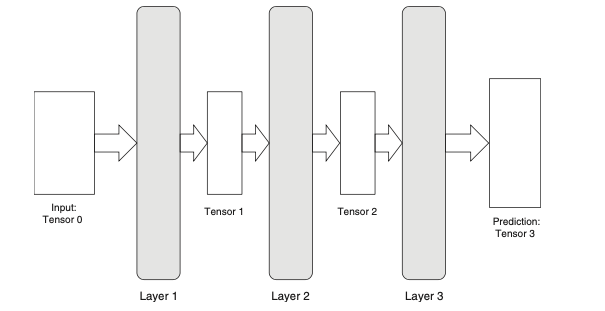
\includegraphics[width=13cm]{kapitel5/tflayers.png}
     \caption[Die Darstellung eines Deep Learning Modells in Tensorflow]{Die Darstellung eines Deep Learning Modells in Tensorflow - Die Tensoren fließen durch jede Schciht im Modell durch (Abbildung aus)}
     \label{Kap5:tnflayers}
 \end{figure}


Im Kern wurde TensorFlow sehr allgemein und flexibel konzipiert: Die Operationen können beliebige genau definierte mathematische Funktionen sein, nicht nur Schichten neuronaler Netze. Dies können beispielsweise mathematische Operationen auf niedriger Ebene sein, beispielsweise das Addieren und Multiplizieren von zwei Tensoren - die Art von Operationen, die innerhalb einer neuronalen Netzwerkschicht stattfinden. Dies gibt Deep-Learning-Ingenieuren und -Forschern die Möglichkeit, beliebige und neuartige Operationen für Deep-Learning zu definieren. Für einen großen Teil der Deep-Learning-Praktiker ist die Manipulation solcher Maschinen auf niedriger Ebene jedoch schwieriger als es sich lohnt. Dies führt zu aufgeblähtem und fehleranfälligerem Code und längeren Entwicklungszyklen. Die meisten Deep-Learning-Ingenieure verwenden eine Handvoll fester Schichttypen (z. B. Faltung, Pooling oder Dichte). In seltenen Fällen müssen neue Ebenentypen erstellt werden. Hier ist die LEGO-Analogie angebracht. Bei LEGOs gibt es nur wenige Blocktypen. LEGO Builder müssen nicht darüber nachdenken, was nötig ist, um einen LEGO Block zu erstellen. Dies unterscheidet sich von einem Spielzeug wie beispielsweise Play-Doh, das der Low-Level-API von TensorFlow entspricht.

Die Fähigkeit, LEGO-Blöcke zu verbinden, führt jedoch zu einer kombinatorisch großen Anzahl von Möglichkeiten und einer praktisch unendlichen Leistung. Es ist möglich, ein Spielzeughaus mit LEGOs oder Play-Doh zu bauen. Wenn Sie jedoch keine besonderen Anforderungen an Größe, Form, Textur oder Material des Hauses haben, ist es viel einfacher und schneller, es mit LEGOs zu bauen. Für die meisten von uns wird das LEGO-Haus, das wir bauen, stabiler stehen und schöner aussehen als das Play-Doh-Haus, das wir bauen würden.

In der Welt von TensorFlow ist das LEGO-Äquivalent die High-Level-API namens Keras.  Keras bietet eine Reihe der am häufigsten verwendeten Arten von neuronalen Netzwerkschichten mit jeweils konfigurierbaren Parametern. Außerdem können Benutzer die Schichten miteinander verbinden, um neuronale Netze zu bilden. Darüber hinaus enthält Keras auch APIs für

\begin{itemize}
     \item Festlegen, wie das neuronale Netzwerk trainiert werden soll (Verlustfunktionen, Metriken und Optimierer)
     \item Daten einspeisen, um das neuronale Netzwerk zu trainieren oder auszuwerten oder das Modell zur Inferenz zu verwenden
     \item Überwachung des laufenden Schulungsprozesses (Rückrufe)
     \item Modelle speichern und laden
     \item Drucken oder Plotten der Architektur von Modellen
 \end{itemize}



Mit Keras können Benutzer den gesamten Deep-Learning-Workflow mit sehr wenigen Codezeilen ausführen. Mit der Flexibilität der Low-Level-API und der Verwendbarkeit der High-Level-API bilden TensorFlow und Keras ein Ökosystem, das im Bereich der Deep-Learning-Rahmenbedingungen hinsichtlich der industriellen und akademischen Akzeptanz führend ist. Als Teil der anhaltenden Deep-Learning-Revolution sollte ihre Rolle, Deep Learning einem breiteren Publikum zugänglich zu machen, nicht unterschätzt werden. Vor Frameworks wie TensorFlow und Keras konnten nur diejenigen mit CUDA-Programmierkenntnissen und umfassender Erfahrung im Schreiben neuronaler Netze in C++ praktisches Deep Learning durchführen. Mit TensorFlow und Keras ist es viel weniger erforderlich, GPU-beschleunigte tiefe neuronale Netze zu erstellen.

Es gab jedoch ein Problem: Es war nicht möglich, TensorFlow- oder Keras-Modelle in JavaScript oder direkt im Webbrowser auszuführen. Um Deep-Learning-Modelle im Browser bereitzustellen, musste dies über HTTP-Requests an einen Backend-Server getan werden. TensorFlow.js löst dieses Problem. Die JavaScript-API hat eine Keras-ähnliche High-Level-API welches auf dem Low-Level-Kern erstellt wurde, die es Benutzern erheblich erleichtert, Deep-Learning-Modelle in der JavaScript-Bibliothek zu definieren, zu trainieren und auszuführen. Um die Interoperabilität weiter zu verbessern, wurden Konverter erstellt, mit denen TensorFlow.js aus TensorFlow und Keras gespeicherte Modelle importieren und Modelle in diese exportieren kann.


\textit{Google Colab} ist ein kostenloser Cloud-Dienst auf Basis von Jupyter Notebooks, der GPU unterstützt. Dies ist nicht nur ein  Tool zur Verbesserung der Codierungsfähigkeiten, sondern ermöglicht es auch absolut jedem, Deep-Learning-Anwendungen mit gängigen Bibliotheken wie PyTorch, TensorFlow, Keras und OpenCV zu entwickeln.

 \begin{figure}[H]
     \centering
     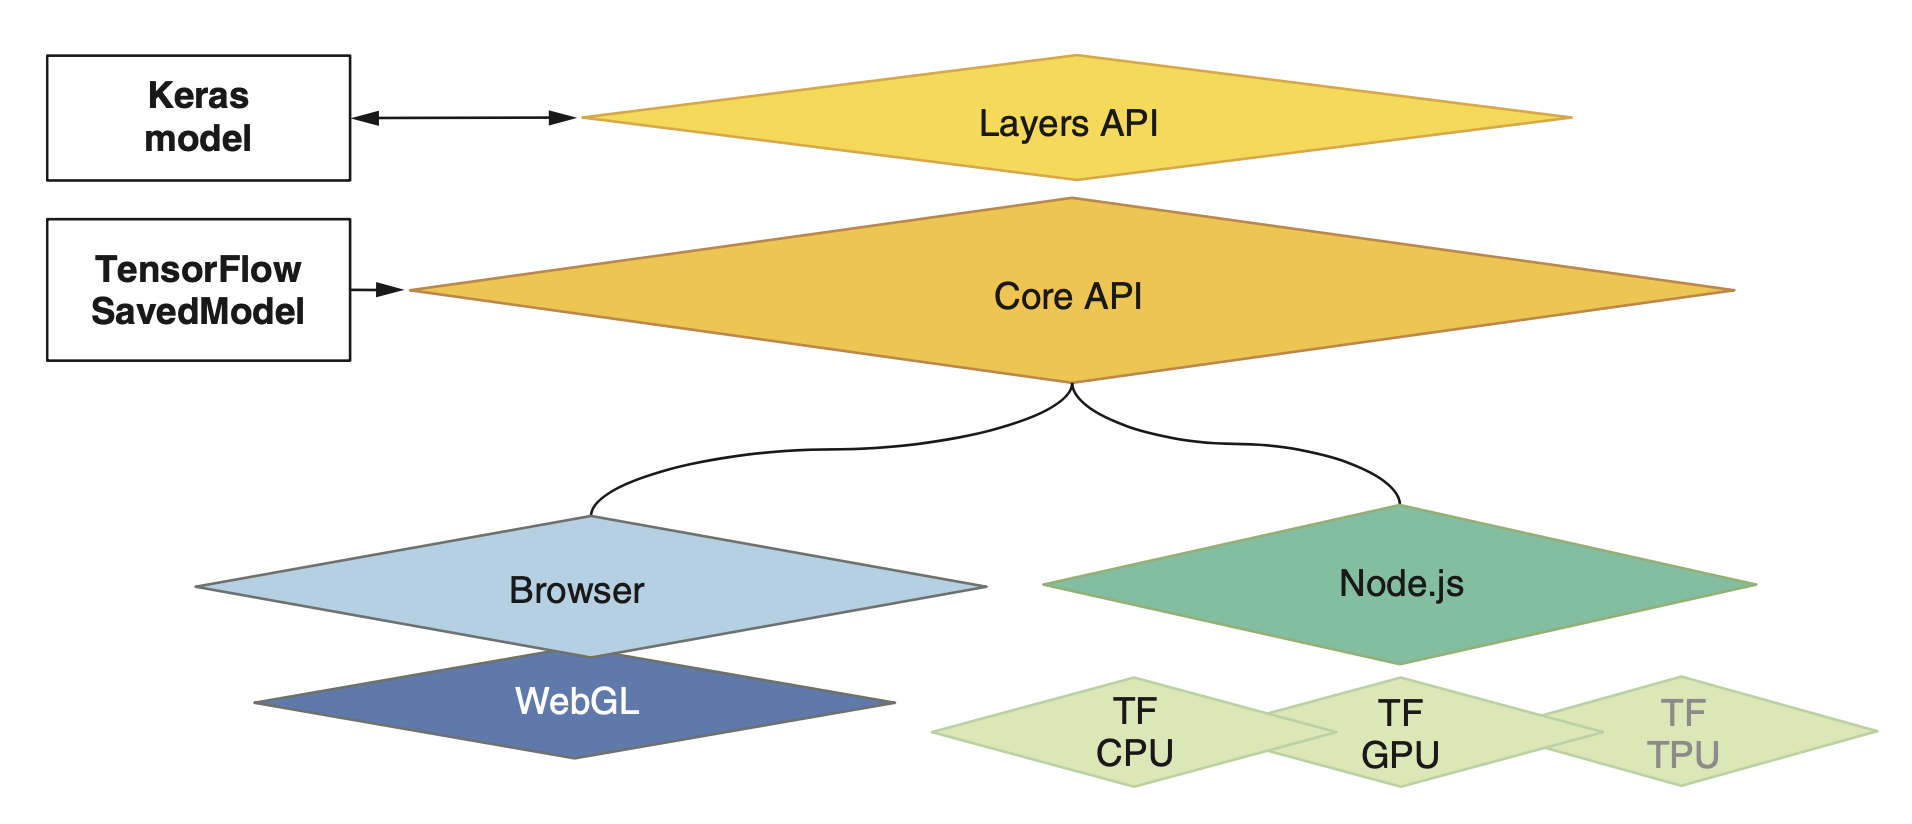
\includegraphics[width=12cm]{kapitel5/tfjsarch.png}
     \caption[Die Architektur von TensorFlow.js]{Die Architektur von TensorFlow.js - Abbildung zeigt die Verhältnisse zwischen der Paython API von TensorFlow und Keras mit TensorFlow.js}
     \label{Kap5:tfjsarch}
 \end{figure}

\section{Preporcessing}
Beim Preprocessing der Daten sollte der Text umgewandelt werden, sodass ein Training erfolgen kann. Bei der Erstellung des Datensatzes wurden die Titel weitestgehend gesäubert. Bei einigen Schlagzeilen waren neben dem Titel auch Namen der Seite vorhanden, diese wurden entfernt. Jedoch sollte der Text, wenn noch nicht erfolgt, in Kleinbuchstaben umgewandelt werden. Die Leerzeichen nach und vor dem jeweiligen Satzzeichen sollte getrennt werden. Da bei Clickbaits Satzzeichen wie Fragezeichen oder Ausrufezeichen eine Beudeutung hat werden diese nicht vollständig entfernt und in den Vokabular aufgenommen. Stoppwörter sind bieten normalerweise keine große Relevanz, sind hier jedoch bedeutsam, z.B. Präpositionen.

Beim Preprocessing wird auch der Datensatz in zwei Hälften, des Trainingssatz und des Testsatz aufgeteilt. Es ist üblich dieses in einer Ratio von 0.8/0.2 auszuführen. Das Ziel ist es vorherzusagen, ob eine bestimmte Schlagzeile Clickbait ist oder nicht. Dieses Bedeutet, dass nach der Entwicklung des Modells Vorhersagen über neue Textüberprüfungen getroffen werden muss. Dieses erfordert, dass für diese neue Überprüfung dieselbe Datenvorbereitung durchgeführt wird, wie für die Trainingsdaten für das Modell. Um sicherzustellen, dass diese Einschränkungen in die Bewertung der Modelle integriert wird, wird vor jeder Datenaufbereitung der Datensatz, in Trainings- und Testsatz aufgeteilt. In der Funktion~\ref{TrainTestFunc} wird der Datensatz aus einer CSV-Datei gelesen und mittels Pandas in ein Dataframe umgewandelt. Es werden zufällig 80\% der Titel \enquote{maskiert} und entsprechend aufgeteilt und als Tupel zurückgegeben. Es entstehen somit ca. 16.000 Beispiele für das Training und 4.000 Beispiele für das Testen.

\begin{lstlisting}[language=Python,caption=Funktion für das Aufteilen des Datensatzes, label={TrainTestFunc}]
import pandas as pd
import numpy as np


def create_train_test(csv_file_path):
    dataframe_ = pd.read_csv(csv_file_path).drop_duplicates()
    msk = np.random.rand(len(dataframe_)) < 0.8
    train = dataframe_[msk]
    test = dataframe_[~msk]
    test.reset_index(drop=True)
    train.reset_index(drop=True)
    return train, test;
\end{lstlisting}

Im Listing~\ref{CleanFunct} werden die Buchstaben in klein gesetzt und alles was nicht gewünscht wird entfernt. Um die Fragezeichen und Ausrufezeichen wird ein Leerzeichen gesetzt, damit diese vom jeweilligen Wort getrennt werden können. Auf das Entfernen der Stoppwörter wird verzichtet, da diese wichtige Informationen über Clickbaits Schlagzeilen geben können.

\begin{lstlisting}[language=Python,caption=Die Preprocessing-Funktion, label={CleanFunct}]
import re


def text_cleaner(text):
    newtext = re.sub(r"[^A-Za-z?!.0-9üäöß]+", " ", text)
    newtext = re.sub("([!?])", r" \1 ", newtext)
    newtext = re.sub("\s{2,}", " ", newtext)
    return newtext.lower()
    
    
train["Title"] = train["Title"].apply(lambda x: text_cleaner(x))
test["Title"] = test["Title"].apply(lambda x: text_cleaner(x))
\end{lstlisting}

\section{Das Erstellen eines Vokabulars}


Es ist wichtig ein Vokabular bekannter Wörter zu definieren, wenn One-Hot-Encoding oder ein Einbettungsmodell verwendet wird. Je mehr Wörter vorhanden sind, desto größer ist die Darstellung von Dokumenten. Daher ist es wichtig, die Wörter nur auf diejenigen zu beschränken, von denen angenommen wird, dass sie vorhersagbar sind. Dies ist im Voraus schwer zu wissen und oft ist es wichtig, verschiedene Hypothesen zum Aufbau eines nützlichen Vokabulars zu testen. Aus dem vorherigen Abschnitt wurde einige Interpunktion (alles außer Fragenzeichen und Ausrufezeichen und Punkt) entfernt. Zahlen wurden nicht entfernt und auch Stoppwörter sind dem Datensatz enthalten. Es kann also aus allen Schlagzeilen eine Reihe aller bekannten Wörter ermittelt werden. Jedes Element im Vokabular wird als Zahl dargestellt. Es handelt sich also um eine Wörterbuchzuordnung von Wörtern und deren Index. Somit kann das Wort auf eine einfache Weise aktualisiert und abgefragt werden.

Keras bietet eine Klasse namens \texttt{Tokeniser} welches diesem Zwecke dient. Diese Klasse ermöglicht die Vektorisierung eines Textkorpus, indem jeder Text entweder in eine Folge von Ganzzahlen (jede Ganzzahl ist der Index eines Tokens in einem Wörterbuch) oder in einen Vektor umgewandelt wird, in dem der Koeffizient für jedes Token basierend auf der Wortanzahl binär sein kann. Der Tokeniser basiert auf der tf-idf Methode.

Die Methode \texttt{fit\_on\_texts} dieser Klasse wird aktualisiert den internen Wortschatz anhand einer Liste von Texten. Um den Text in eine Folge von ganzen Zahlen umzuwandeln ist das Ausführen der Methode \texttt{fit\_on\_texts} zwingend erforderlich. Dann kann mit der Methode \texttt{texts\_to\_sequences} die häufigsten auftretenden Wörter die dem Tokeniser bekannt sind berücksichtigt.

Der nächste Schitt ist das Padding. Mit der Methode \texttt{pad\_sequences} kann eine Liste von Sequenzen mit einer bestimmten Länge in ein 2-Dimensionales-Numpy-Array umgewandelt werden. Sequenzen die länger als die angegebene maximale Länge sind werden abgeschnitten, damit sie der gewünschten Länge entsprechen. Sequenzen die kürzer sind wiederum, werden mit einer Null aufgefüllt, bis sie dem maximalen Wert entsprechen. Das Vorabfüllen oder Entfernen von Werten am Anfang der Sequenz ist die Standardeinstellung. Es wird festgestellt, dass die Titel im Datensatz eine maximale Tokenlänge von 21 haben. Die maximale Länge wird auf 40 Tokens gesetzt. Es wird also nachher erlaubt, eine Abfrage mit maximal 40 Wörtern oder Tokens durchzuführen. Der Tokeniser gibt somit z.B. für den Titel \enquote{die 10 besten apps für mädchen} einen Array der Länge 30, wobei die ersten 24 Werte eine Null enthalten und die restlichen 6 eine bestimmte Zahl, welches den Index des im String enthaltenen Wörtes darstellt. 



\begin{lstlisting}[language=Python,caption=Die Tokeniser-Funktion, label={TokenizerFunc}]
from keras.preprocessing.text import Tokenizer
from keras.preprocessing.sequence import pad_sequences


def tokenize_text(train_df, test_df, max_l):
    tokenizer = Tokenizer(filters='"#$%&()*+-/:;<=@[\\]^_`{|}~\t\n')
    tokenizer.fit_on_texts(train_df)
    vocab_size = len(tokenizer.word_index) + 1
    tokenized_text_train = pad_sequences(
        tokenizer.texts_to_sequences(train_df), maxlen=max_l)
    tokenized_text_test = pad_sequences(
        tokenizer.texts_to_sequences(test_df), maxlen=max_l)
    return {"tokenized_text_train": tokenized_text_train, "tokenized_text_test": tokenized_text_test, "vocab_size": vocab_size, "tokenizer": tokenizer}
\end{lstlisting}

%Es basiert auf TFIDF ==> aufmahme in den teoretischen Teil
% curse of dimeniolaty in teoretischen teil nehmen
% FOrmel sind nicht on flow mit den zahlen

Eine Worteinbettung ist eine Möglichkeit, Text darzustellen, bei der jedes Wort im Vokabular durch einen reellen Vektor in einem hochdimensionalen Raum dargestellt wird. Die Vektoren werden so gelernt, dass Wörter mit ähnlichen Bedeutungen eine ähnliche Darstellung im Vektorraum haben (nahe im Vektorraum). Dies ist eine aussagekräftigere Darstellung für Text als klassische, bei denen Beziehungen zwischen Wörtern oder Token ignoriert oder in Bigram- und Trigramm-Ansätzen erzwungen werden. Die Vektordarstellung für Wörter kann während des Trainings des neuronalen Netzwerks gelernt werden. Dieses kann in der Keras Deep Learning-Bibliothek mithilfe der Einbettungsebene ausgeführt werden. 


Die Keras-Einbettungsschicht erfordert Ganzzahl-Eingaben, bei denen jede Ganzzahl einem einzelnen Token zugeordnet ist, das eine bestimmte reelle Vektordarstellung innerhalb der Einbettung aufweist. Diese Vektoren sind zu Beginn des Trainings zufällig, werden jedoch während des Trainings für das Netzwerk von Bedeutung. Durch die Funktionen aus Listing~\ref{CleanFunct} und Listing~\ref{TokenizerFunc} wurde das Encoding ausgeführt. Schließlich werden die Klassenbezeichnungen für den Trainingsdatensatz und Testdatensatz definieren, die für das überwachte neuronale Netzwerkmodell erforderlich sind, um die Clickbaits vorherzusagen. Die Daten werden zuletzt in ein TensorFlow dataset umgewandelt, um sie leichter in Keras einzuspeisen. Somit entsteht ein Datensatz zum training mit einem gesamten Vokabular von ca. 23.000 Vokabeln und einer erwarteten maximalen Eingangslänge von 30 Wörtern.

Die Daten wurden in den frühereren Etappen in \enquote{Train} und \enquote{Test} aufgeteilt. Mit der Funktion aus Listing~\ref{LabelFunc} werden die Labels \textit{Clickbait 0} und  \textit{News 1} in ein Array umgewandelt, um sie später in mittels \texttt{tensorflow\_datasets} umzuwandeln, gemeinsam mit den Arrays der Tokens (siehe Listing~\ref{DataSet)}. Der Grund für diese Konversion ist, dass diese Daten viel einfacher codiert und encodiert werden können, als z.B. mit Pandas Dataframes (siehe Listing~\ref{TrainModel}).


\begin{lstlisting}[language=Python,caption=Die Label-Funktion, label={LabelFunc}]
def create_labels(train_data, test_data):
    encoded_labels = preprocessing.LabelEncoder()
    y = encoded_labels.fit_transform(train_data["label"])
    y = to_categorical(y)
    y_test = encoded_labels.transform(test["label"])
    y_test = to_categorical(y_test)
    return y, y_test;

y, y_test = create_labels(train, test)
\end{lstlisting}

\begin{lstlisting}[language=Python,caption=Die Dataset Erstellung, label={DataSet}]
import tensorflow_datasets as tfds

train_dataset = tf.data.Dataset.from_tensor_slices((tokenized_text_train, y))
test_dataset = tf.data.Dataset.from_tensor_slices((tokenized_text_test, y_test))
\end{lstlisting}





\section{Die Modellarchitektur}



In Listing~\ref{BuildModel} wird ein sequentielles Modell erstellt. Diesem Modell kann durch die Methode \texttt{add} jeweils eine Schicht angehängt werden, und Keras arbeitet dieses nacheinander ab. Die API von Keras von Keras wird verwendet um das Modell zusammen zu bauen. Die Definitionen der einzelnen Methoden mit der das Modell gebaut und trainiert wurde, sind aus der Dokumentation von Google\citep{google1} entnommen. Dort werden viele Begriffe, die im Zusammenhang mit dem bauen und trainieren eines Deep Learning oder Machine Learning Modells stehen erklärt. Aus diesem Grund wird in diesem und nächsten Abschnitt auf diese Quelle verwiesen.

\begin{lstlisting}[language=Python,caption=Das Bilden des Models, label={BuildModel}]
from tensorflow.keras.models import Sequential
from tensorflow.keras.layers import Conv1D, MaxPool1D, Dropout, Dense, GlobalMaxPool1D, Embedding, Activation

def build_model(vocab_size, emb_dim, max_len, dropout_rate, learning_rate, n_labels):
    loss = tf.keras.losses.BinaryCrossentropy()
    metric = [tf.keras.metrics.BinaryAccuracy(name="accuracy")]
    opt = tf.keras.optimizers.Adam(learning_rate=learning_rate)

    model = Sequential([])
    model.add(
        Embedding(vocab_size, output_dim=emb_dim, input_length=max_len))
    model.add(Dropout(dropout_rate))
    model.add(Conv1D(filters=32, kernel_size=8,
                           activation="relu", padding="same", strides=1))
    model.add(GlobalMaxPool1D())
    model.add(Dense(16, activation="relu"))
    model.add(Dense(n_labels, activation="softmax"))
    model.compile(loss=loss, metrics=metric, optimizer=opt)
    model.summary()
    return model
    
model = build_model(vocab_size=vocab_size, emb_dim=32, max_len=40, dropout_rate=0.3, learning_rate=0.00006, n_labels=len(labels))
\end{lstlisting}


Zunächst mussen einige Parameter festgelegt werden. Diese sind \texttt{loss} also die Verlustfunktion, \texttt{metric} also nach welchen Metriken das Modell bemessen werden soll und \texttt{opt} der \texttt{Optimizer} wodurch das Modell lernt. Da es sich um eine binäre Klassifikation handelt wurden diese entsprechend den Parameteren ergänzt. Da es eine binäre Klassifikation ist, wird wird die \texttt{BinaryCrossentropy} verwendet. Als Optimizer wurde \texttt{Adam} ausgewählt. Die Lernrate ist ein Skalar, mit dem ein Modell über einen Gradientenabstieg trainiert wird. Während jeder Iteration multipliziert der Gradientenabstiegsalgorithmus die Lernrate mit dem Gradienten. Das resultierende Produkt wird als Gradientenschritt bezeichnet. Die Lernrate ist ein wichtiger Hyperparameter. Ein Optimizer ist eine spezifische Implementierung des Gradientenabstiegsalgorithmus. Die Basisklasse von TensorFlow für Optimierer ist tf.train.Optimizer. Beliebte Optimierer sind \texttt{AdaGrad}, das für ADAptive GRADient Abstammung steht und \texttt{Adam}, der für ADAptive with Momentum steht. Hyperparameter können dafür verwendet werden, um das Modell zu justieren und es gibt keine wirklichen Regel bei dem Konsum dieser Paramater. 

Nachdem die Hyperparameter popularisiert wurden, wird dem Modell die erste Schicht zugeführt. Dieses ist die Einbettungsschicht. Die Worteinbettung sind eine Möglichkeit, ein Wort als Vektor darzustellen (ein 1D-Tensor in TensorFlow). Durch Worteinbettungen können jedoch die Werte der Elemente des Vektors trainiert werden, anstatt nach einer Regel wie der Wort-zu-Index-Zuordnung in One-Hot-Codierung fest codiert zu werden. Mit anderen Worten, wenn ein textorientiertes neuronales Netzwerk die Worteinbettung verwendet, werden die Einbettungsvektoren zu trainierbaren Gewichtungsparametern des Modells. Sie werden durch dieselbe Backpropagation-Regel wie alle anderen Gewichtungsparameter des Modells aktualisiert. Es gibt auch die Möglichekeit, eine vortrainierte Einbettungsschicht zu nehmen. Diese werden auf viel größere Mengen an Daten trainiert und können für vielseitige Zwecke verwendet werden, ohne dass von Grunde aus neu trainiert werden muss. In diese Fall trainiert das Modell die Einbettungen selbst, anstatt sich auf die vorab trainierten Einbettungen zu verlassen.


Um das Modell vor dem Overfitting zu schützen gibt es bestimmte Strategien, die angewendet werden können. Dieses sind sogenannte Regularisierungstrategien. Es kann als eine Art \enquote{Strafe} betrachtet werden, für die Komplexität des Modells. Da bei wenig Daten und hoher Komplexität das Modell nicht wirklich lernt, sondern sich den gegebenen wenigen Daten \enquote{überanpasst} können diese dagegen wirken. 


Wenn Neuronen Muster in Trainingsdaten vorhersagen, indem sie sich fast ausschließlich auf Ausgaben bestimmter anderer Neuronen stützen, anstatt sich auf das Verhalten des Netzwerks als Ganzes zu verlassen, entsteht eine Anpassung. Wenn die Muster, die eine Anpassung verursachen, nicht in den Validierungsdaten vorhanden sind, weil es zu wenig Daten gibt, führt dies zu einer Überanpassung. Die Dropout-Regularisierung reduziert die Co-Anpassung, da Dropout sicherstellt, dass sich Neuronen nicht nur auf bestimmte andere Neuronen verlassen können. Die Dropout-Regularisierung entfernt eine zufällige Auswahl einer festen Anzahl von Einheiten in einer Netzwerkschicht für einen einzelnen Gradientenschritt. Je mehr Einheiten ausfielen, desto stärker war die Regularisierung. 



Die \texttt{Conv1D}-Ebene wird verwendet um die Faltung durchzuführen. Eine CNN ist ein neuronales Netzwerk, in dem mindestens eine Schicht die Faltungsschicht ist. Ein typisches neuronales Faltungsnetzwerk besteht aus einer Kombination der von Faltungsschichten, Poolingschichten, und vollständig verbundene Schichten. Die Faltungsschicht hier ist eine eindimensionale Faltungsschicht. Bestimmte Muster aus dem Text werden hier erkannt (z.B. ob nach einem negativen Verb ein bestimmtes Wort auftaucht. In dem Beispiel gibt es 32 Filter. Beim maschinellen Lernen werden Faltungsfilter normalerweise mit Zufallszahlen gesetzt, und dann trainiert das Netzwerk die idealen Werte. Die \textit{kernel\_size} ist eine Zahl, die die Höhe des Faltungsfensters angibt. Zusätzlich zur eindimensionalen Faltungsschicht wird eine ebenfalls eindimensionale Poolingsschicht zugeführt.


Die \texttt{Dense}-Schichten sind verborgene Schichten, in der jeder Knoten mit jedem Knoten in der nachfolgenden verborgenen Schicht verbunden ist. Eine vollständig verbundene Schicht wird auch als dichte Schicht \enquote{dense layer} bezeichnet. Das erste der beiden Schichten im Modell hat 16 Einheiten und das zweite hat genau so viele Einheiten wie es Labels gibt (dieses Modell hat genau 2, da es 2 Klassen gibt), da sie die letzte Schicht ist.

Eine Aktivationsfunktion (z. B. ReLU oder Sigmoid), die die gewichteten Summen aller Eingaben aus der vorherigen Ebene. Sie werden als Ausgabewert (normalerweise nichtlinear) generiert und an die nächste Ebene weiterleitet. Die ReLu fungiert mit folgenden Regeln: wenn der Eingang negativ oder Null ist, ist der Ausgang 0 und wenn der Eingang positiv ist, ist der Ausgang gleich dem Eingang. Die softmax-Funktion, ist eine Funktion, welches die Wahrscheinlichkeiten für jede mögliche Klasse in einem Klassifizierungsmodell mit mehreren Klassen bereitstellt. Die Wahrscheinlichkeiten summieren sich auf genau 1,0. Zum Beispiel könnte softmax bestimmen, dass die Wahrscheinlichkeit, dass ein bestimmtes Bild ein Hund bei 0,9, eine Katze bei 0,08 und ein Pferd bei 0,02 ist.

Mit der \texttt{compile}-Methode lässt sich das Modell bauen und die \texttt{summary}-Methode gibt eine Übersicht über das Modell (siehe Tabelle~\ref{modellBesch}).


\begin{table}[h]
    \caption{Beschreibung der Schichten des Modells}
    \label{modellBesch}
    \renewcommand{\arraystretch}{1.2}
    \centering
    \sffamily
    \begin{footnotesize}
        \begin{tabular}{l l l}
            \toprule
            \textbf{Layer (type)}                  & \textbf{Output Shape} & \textbf{Param \#} \\
            \midrule
            embedding (Embedding)  & (None, 40, 32) & 740384                \\
            dropout (Dropout)  & (None, 40, 32) &     0      \\
            conv1d (Conv1D)                  & (None, 40, 32)     &    8224     \\
            global\_max\_pooling1d (GlobalMaxPool1D)   & (None, 32)                    &     0   \\
            dense (Dense)    & (None, 16)     &  528      \\
            dense (Dense)   & (None, 2)     & 34                      \\
            \bottomrule
        \end{tabular}
    \end{footnotesize}
    \rmfamily
\end{table}

\section{Das Training}

Mit der Funktion \texttt{train\_model} aus Listing~\ref{TrainModel} lässt sich das Modell trainieren. Zunächst muss als Parameter angegeben werden, wie viele Trainingsepochen das Modell trainiert werden soll. Ein vollständiger Trainingsdurchlauf über den gesamten Datensatz, sodass jedes Beispiel einmal gesehen wurde wird als Epoche genannt. Die \texttt{batch\_size} sind die Anzahl der Beispiele in einer Charge/Epoche. Vor dem Training bietet sich die Möglichkeit, die Daten zu mischen, dieses erfolgt mit dem Parameter \textit{shuffle}. Analysen über das Training kann mit TensorBoard durchgeführt werden. TensorBoard bietet die Visualisierung und Werkzeuge, die für Experimente mit maschinellem Lernen erforderlich sind. Metriken wie Verlust und Genauigkeit können mit TensorBoard für jede Epoche dargestellt werden. Damit TensoBoard im späteren Verlauf verwendet werden kann, wird eine Callback-Funktion eingebaut, welches den Verlauf des Trainings in Logdateien speichert. Mit der \textit{fit}-Methode erfolgt das Training (siehe Listing~\ref{TrainModel}).


\begin{lstlisting}[language=Python,caption=Das Training des Models, label={TrainModel}]
import os
import datetime

def train_model(num_epochs, batch_size, train_ds, test_ds, model, shuffle):
    ds_train_encoded = train_ds.shuffle(shuffle).batch(batch_size)
    ds_test_encoded = test_ds.batch(batch_size)
    logdir = os.path.join(
        "logs", datetime.datetime.now().strftime("%Y%m%d-%H%M%S"))
    tensorboard_callback = tf.keras.callbacks.TensorBoard(
        logdir, histogram_freq=1)
    model.fit(ds_train_encoded, epochs=num_epochs,
              validation_data=ds_test_encoded, callbacks=[tensorboard_callback])
    
train_model(num_epochs=7, batch_size=32, train_ds=train_dataset, test_ds=test_dataset, model=model, shuffle=1000)
\end{lstlisting}





\section{Evaluation}\label{evaSec}

Das sogennante \enquote{cross validation} ist ein Mechanismus zum Schätzen, wie gut sich ein Modell auf neue Daten verallgemeinern lässt, indem das Modell anhand einer oder mehrerer nicht überlappender Datenuntergruppen getestet wird, die aus dem Trainingssatz zurückgehalten werden. Mit der Bibliothek \enquote{sklearn} können mit der Methode \texttt{classification\_report} einen Textbericht mit den wichtigsten Klassifizierungsmetriken erstellt werden. Dieser Report gibt Auskünft über bestimmte Metriken, mit der das Performance des Modells auf den vorhandenen Daten gemessen werden kann. 

\begin{lstlisting}[language=Python,caption=Das Evaluieren des Models, label={TrainModel}]
import numpy as np
from keras.utils import to_categorical
from sklearn.metrics import classification_report

y_pred = to_categorical(np.argmax(
    model.predict(tokenized_text_test), axis=1))

print(classification_report(y_test, y_pred, target_names=labels.values(), digits=4))
\end{lstlisting}



\begin{table}[h]
    \caption{Die Ergebnisse der Evaluation des Modells}
    \label{eval1}
    \renewcommand{\arraystretch}{1.2}
    \centering
    \sffamily
    \begin{footnotesize}
        \begin{tabular}{l l l l l}
            \toprule
                           & \textbf{precision} & \textbf{recall} & \textbf{f1-score} & \textbf{support} \\
            \textbf{Clickbaits} & 0.9775                  & 0.9589                 & 0.9681                & 1993          \\
            \textbf{News}  & 0.9590                 & 0.9776                & 0.9682               & 1961                     \\
            \bottomrule
        \end{tabular}
    \end{footnotesize}
    \rmfamily
\end{table}

\begin{figure}[H]
    \centering
    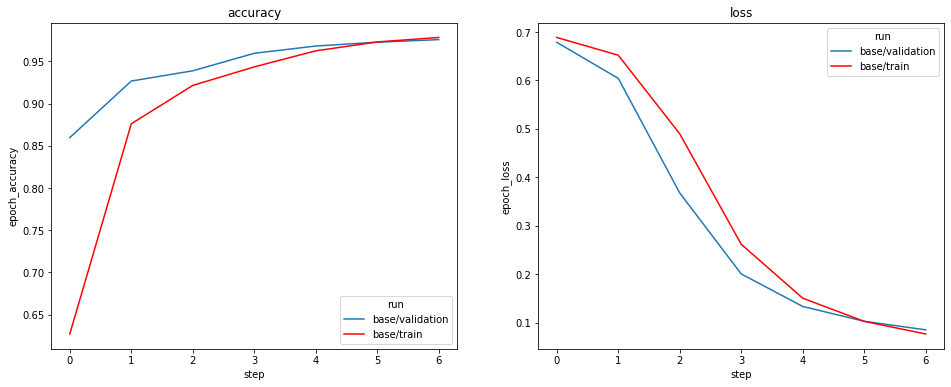
\includegraphics[width=15cm]{kapitel5/basemodel.png}
    \caption[Vergleich der Genauigkeit mit dem Verlust]{Blau: Validationsdaten. Rot: Trainingsdaten. Links: Die Genauigkeit der Trainings- und Testdatensätze kommt mit jeder Epoche näher und steigt. Rechts: Beide Verlustfunktionen nehmen ab. Während aller Epochen ist eine leichte Überanpassung zu sehen, welches jedoch immer mehr ausgeglicehener wird.}
    \label{Kap5:Val}
\end{figure}



Im praktischen Gebrauch wird das Modell nicht so gute Performance bringen, wie mit den kleinen Mengen an Daten. Es gibt in der Realität weitaus mehr Webseiten als die im Datensatz. Oft ist auch der Kontext entscheidend. Es ist unmöglich, ein Modell zu entwickeln, welches auf diese Gegebenheiten trainiert wurde. Zum Abschluss dieses Abschnittes sollen einige \enquote{Schwachstellen} dieses Modells mittels praktischer Anwendung dargestellt werden. Es können \enquote{offentsichtliche} Clickbaits und Nachrichten in das Modell eingegeben werden, um zu sehen, ob es eine falsche Vorhersage ausübt.


Zunächst muss der Text der als String eingegeben wird in Tokens umgewandelt. Dann muss diese Sequenz, unter berücksichtigung der maximalen Länge, das Padding, also das zuführen von Nullen, durchgeführt werden. Wenn der Text in Zahlen umgewandelt wurde kann die Methode \texttt{predict} benutzt werden um Vorhersagen auszuüben. Diese Methode gibt für jeden eingegebenen Satz ein numpy Array zurück welches in numpy \texttt{argmax} eingegeben wird. Somit wird am Ende für die Indizes die Maximalwerte entlang einer Achse zurückgegeben. Das Ergebnis wird in der Tabelle~\ref{PredictNewTab} dargestellt.


\begin{table}[h]
    \caption{Vorhersagen des Modells für neue Schlagzeilen}
    \label{PredictNewTab}
    \renewcommand{\arraystretch}{1.2}
    \centering
    \sffamily
    \begin{footnotesize}
        \begin{tabular}{l l}
            \toprule
            \textbf{Schlagzeile}                  & \textbf{Vorhersage} \\
            \midrule
            Die 10 lustigsten Bilder von Katzen! & Clickbait \\
            Diese Rezepte solltest du nicht verpassen!  & Clickbait    \\
            Aus diesem Grund sollten Sie ihr Smartphone während des Schlafens ausschalten                  & Clickbait       \\
            13 Dinge, die Sie garantiert noch nicht über ihr Smartphone wussten   & Clickbait                   \\
            Sondersitzung des Kabinetts - Bayern ruft erneut Katastrophenfall aus   & News        \\
            Russland verschärft Ton im Pipeline-Streit  & News                     \\
            Nordkorea präsentiert offenbar modernisierte Raketentypen & News \\
            „Wandelnde Arzneimittelwerbung“ als Kanzlerkandidat? & News \\
            Corona im News-Ticker: RKI meldet über 2 Mio. Infektionen - droht Mega-Lockdown? & Clickbait \\
            Die 7 besten Tageslinsen 2021 im Vergleich & Clickbait \\
            Er hatte alles – nur ein Erbe fehlte ihm: Zum Tod von Modegenie Pierre Cardin & Clickbait \\
            „Pass mal auf“: Lanz fragt nach Tempolimit 130, Merz knallt ihm einen vor den Latz & News \\
            Trump ist ein Politverbrecher wie Putin oder Erdoğan & Clickbait \\
            Wie Kinder die Corona-Pandemie beeinflussen & Clickbait \\
            Was steht in den Impfstoff-Verträgen? & Clickbait \\
            \bottomrule
        \end{tabular}
    \end{footnotesize}
    \rmfamily
\end{table}

In der Tabelle~\ref{PredictNewTab} sind die Ergebnisse des Experiments aus dem Listing~\ref{PredictNew}. Es lassen sich bestimmte Muster erkennen. Offentsichtliche Clickbaits und Nachrichten (die ersten 8 Schlagzeilen) werden gut erkannt. In diesen 8 Schlagzeilen haben Clickbaits die Eigenschaft, eine Zahl zu beinhalten und relativ kurze Wortlängen zu haben. Außerdem ist deutlich zu sehen, dass bei den Nachrichten sich um Internationale Themen handelt und lange Wörter wie \enquote{Kanzlerkandidat} vorhanden sind.

Das Modell kann aber auch falsch Alarm schlagen. Wie im Beispiel \enquote{Corona im News-Ticker: RKI meldet über 2 Mio. Infektionen - droht Mega-Lockdown?}, zwar ist hier ein Wort \enquote{Mega} welches ein oft in Clickbaits verwendetes Wort ist und auch eine Zahl (2) ist enthalten, ebenfalls wird eine Frage gestellt. Das Modell kann aber nicht erkennen, bzw. weiß nicht, dass diese Mittel (das Stellen einer Frage, verwenden von Zahlen usw.) auch in konventionellen Nachrichten verwendet werden. Hier wird deutlich, dass alleine die Überprüfung des Titels der Nachricht, auch zu falschen Ergebnissen führen kann. Es sollte ebenfalls der Inhalt der Nachricht überprüft und aus dem Zusammenhang beider Ergebnisse eine Vorhersage gemacht werden. Es ist jedoch auffällig, dass das Modell Schwierigkeiten hat Nachrichten zu erkennen aber weniger Probleme damit hat, Clickbaits zu erkennen. Dieses könnte daran liegen, dass Nachrichten oft falsch intrepetiert werden können, weil sie bestimmte Eigenschaften haben, die in Clickbaits vorhanden sind.

\section{Experimente}

Wie im Abschnitt~\ref{overundersec} beschrieben ist die Über- bzw. Unteranpassung zu vermeiden. Zwar gibt es Strategien wie im Abschnitt~\ref{regSec} definiert, aber auch die Anpassung der Hyperparameter wie die Lernrate können wichtige Auswirkungen auf das Kriterium der Über- oder Unteranpassung haben. Ein weiteres Experiment kann gemacht werden, welches die Lernrate und die Auswirkung der Lernrate( im Abschnitt~\ref{learnsection} näher beschrieben), untersucht. Das Ziel dieser Experimente soll dabei Untersuchen, ob und wie sich das Modell ändert. Das Modell aus Tabelle~\ref{modellBesch} hat 32 Einbettungsdimensionen. Die Lernrate beträgt 0.00006 und sie hat eine Dropout-Rate von 0.35. Ziel ist es zu sehen, ob das Modell besser performt oder nicht und dabei nicht eine Überanpassung entsteht. Das Modell liefert zwar gute Ergebnisse, aber es sollte betrachtet werden, dass der Datensatz relativ klein ist und das Modell bei einem größeren Datensatz nicht so gut performen könnte. Folgende Fragen werden mit 3 Experimenten näher betrachtet.

\paragraph{Die Veränderung der Einbettungsdimension}
Die Einbettungsdimension ist der Parameter, der über die Dimensionalität der Einbettung entscheidet. Je größer diese Dimension ist, desto mehr Parameter sollten entstehen, da das Modell diese Einbettungen lernen muss. Somit würde vom Volumen her ein größeres Modell entstehen, welches bei gleicher Performance vermieden sollte. Dieser Parameter wird von 32 auf 320 gesetzt. Alle anderen Parameter wurde nicht verändert. An der Performance ändert sich wenig (siehe Tabelle~\ref{eval32}) jedoch entsteht eine Überanpassung ab der 3. Epoche des Trainings (siehe Abbildung~\ref{32embdpic}).

\begin{table}[h]
    \caption{Die Ergebnisse des Modells mit 320 Einbettungsdimensionen}
    \label{eval32}
    \renewcommand{\arraystretch}{1.2}
    \centering
    \sffamily
    \begin{footnotesize}
        \begin{tabular}{l l l l l}
            \toprule
                           & \textbf{precision} & \textbf{recall} & \textbf{f1-score} & \textbf{support} \\
            \textbf{Clickbaits} & 0.9761                  & 0.9867                 & 0.9814                & 1948          \\
            \textbf{News}  & 0.9869                 & 0.9766                & 0.9817               & 2009                     \\
            \bottomrule
        \end{tabular}
    \end{footnotesize}
    \rmfamily
\end{table}

\begin{figure}[H]
    \centering
    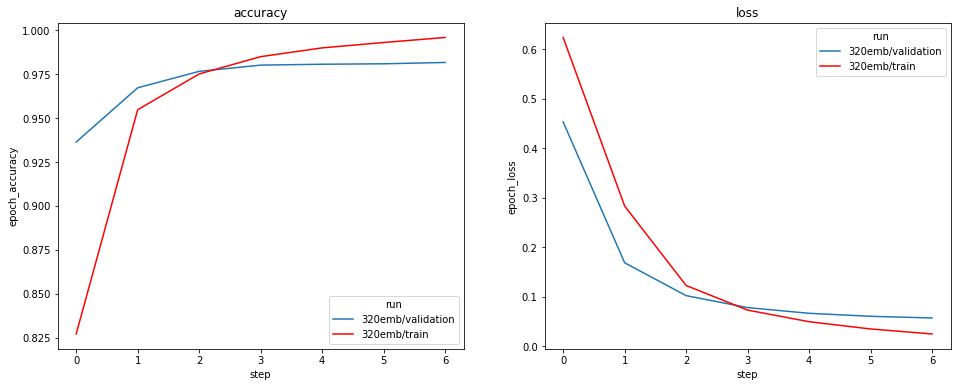
\includegraphics[width=15cm]{kapitel5/320embd.png}
    \caption[Auswirkung der Einbettungsdimensionen]{Ab der 3. Epoche findet eine Überanpassung statt.}
    \label{32embdpic}
\end{figure}

\paragraph{Die Veränderung der Der Lernrate von 0.00006 auf 0.0006}
Im Abschnitt~\ref{learnsection} wurde die Bedeutung der Lernrate im Deep Learning vorgegstellt. Durch die verzehnfachung der Lernrate (von 0.00006 auf 0.0006) lernt das Modell mit einer höheren Rate und es ist in der Abbildung~\ref{learnpic} deutlich zu sehen, dass eine Überanpassung herrscht. 

\begin{table}[h]
    \caption{Die Ergebnisse der Evaluation des Modells mit einer Lernrate von 0.0006}
    \label{evallearn}
    \renewcommand{\arraystretch}{1.2}
    \centering
    \sffamily
    \begin{footnotesize}
        \begin{tabular}{l l l l l}
            \toprule
                           & \textbf{precision} & \textbf{recall} & \textbf{f1-score} & \textbf{support} \\
            \textbf{Clickbaits} & 0.9778                 & 0.9933                 & 0.9855                & 1948          \\
            \textbf{News}  & 0.9934                 & 0.9781                & 0.9857               & 2009                     \\
            \bottomrule
        \end{tabular}
    \end{footnotesize}
    \rmfamily
\end{table}

\begin{figure}[H]
    \centering
    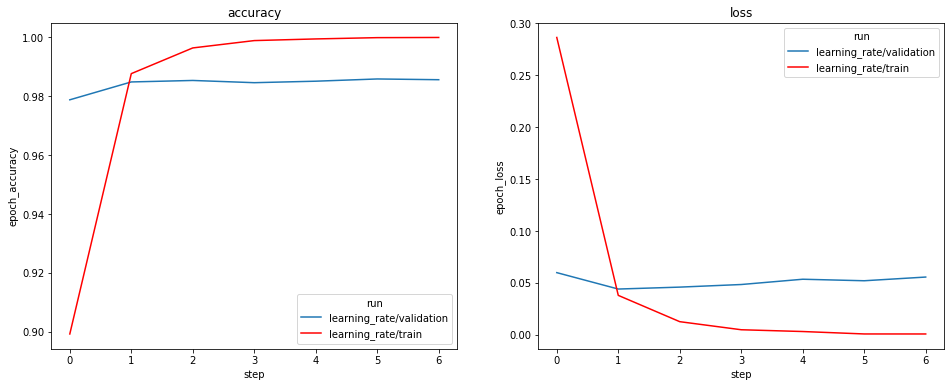
\includegraphics[width=15cm]{kapitel5/learningrate.png}
    \caption[Auswirkung der Lernrate]{Es ist zu sehen, wie das Modell in der ersten Epoche das meiste gelernt hat und sich danach nur noch dem Modell anpasst.}
    \label{learnpic}
\end{figure}

\paragraph{Das Hinzufügen von zusätzlichen Schichten}
Dem Modell aus Tabelle~\ref{modellBesch} werden zusätzliche Conv1D-Schichten hinzugefügt. Zusätzlich werden dem Modell 256 statt 32 Einbettungsdimensionen hinzugefügt. Die Dropout-Rate wird auf 0.1 gesetzt, da dieses Modell mehr Schichten dieser Art besitzt. Die Lernrate bleibt unverändert. Die Schichten werden nach der Beschreibung aus der Tabelle~\ref{modellBesch2} angepasst. Auch hier findet eine \enquote{schnelles Lernen} statt, wie in Abbildung~\ref{extrlayerspic} dargstellt. Es findet auch hier eine Überanpassung statt. Das Modell hat zusätzliche Faltungsschichten (siehe Tabelle~\ref{modellBesch2}) und auch mehr Parameter zum trainieren. Es wurden außerdem 2 zusätzliche Dropout-Schichten hinzugefügt.

\begin{table}[h]
    \caption{Das \enquote{komplexere} Modell}
    \label{modellBesch2}
    \renewcommand{\arraystretch}{1.2}
    \centering
    \sffamily
    \begin{footnotesize}
        \begin{tabular}{l l l}
            \toprule
            \textbf{Layer (type)}                  & \textbf{Output Shape} & \textbf{Param \#} \\
            \midrule
            embedding (Embedding)  & (None, 40, 256) & 6000640                \\
            dropout (Dropout)  & (None, 40, 256) &     0      \\
            conv1d (Conv1D)                  & (None, 40, 50)     &    38450     \\
            max\_pooling (MaxPooling1D)                  & (None, 20, 50)     &0     \\
            dropout (Dropout)  & (None, 20, 50) &     0      \\
            conv1d (Conv1D)                  & (None, 20, 100)     &    15100     \\
            max\_pooling (MaxPooling1D)                  & (None, 10, 100)     &0     \\
            dropout (Dropout)  & (None, 10, 100) &     0      \\
            conv1d (Conv1D)                  & (None, 10, 200)     &    60200     \\
            global\_max\_pooling1d (GlobalMaxPool1D)   & (None, 200)                    &     0   \\
            dropout (Dropout)  & (None, 200) &     0      \\
            dense (Dense)    & (None, 100)     &  20100      \\
            dense (Dense)   & (None, 2)     & 202                      \\
            \bottomrule
        \end{tabular}
    \end{footnotesize}
    \rmfamily
\end{table}

\begin{table}[h]
    \caption{Die Ergebnisse des Modells mit zusätzlichen Schichten}
    \label{eval2}
    \renewcommand{\arraystretch}{1.2}
    \centering
    \sffamily
    \begin{footnotesize}
        \begin{tabular}{l l l l l}
            \toprule
                           & \textbf{precision} & \textbf{recall} & \textbf{f1-score} & \textbf{support} \\
            \textbf{Clickbaits} & 0.9722                  & 0.9887                 & 0.9804                & 1948          \\
            \textbf{News}  & 0.9889                 & 0.9726                & 0.9807               & 2009                     \\
            \bottomrule
        \end{tabular}
    \end{footnotesize}
    \rmfamily
\end{table}


\begin{figure}[H]
    \centering
    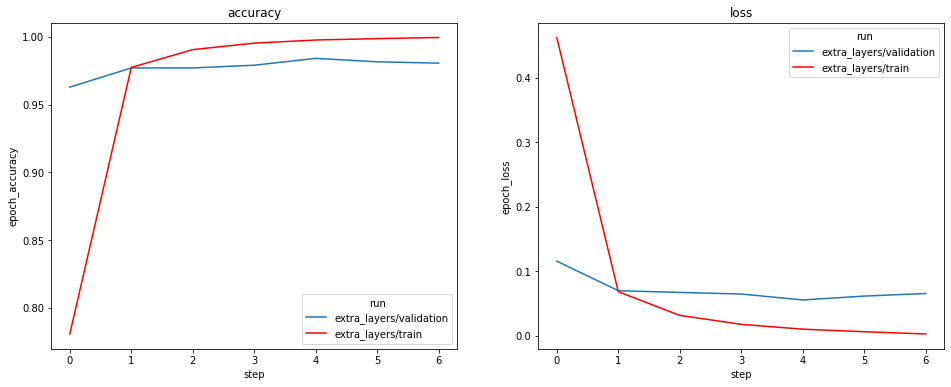
\includegraphics[width=15cm]{kapitel5/complexmodel_.png}
    \caption[Auswirkung der zusätzlichen Schichten]{Das Modell \enquote{lernt schnell} und passt sich früh an die Daten an.}
    \label{extrlayerspic}
\end{figure}

\section{Speichern und Konvertierung des Modells und der Tokens}
Das Keras Modell wird mit als h5-Datei gespeichert. Diese Datei kann mit dem TensorFlow.js Konverter, welches Keras Modelle in für TensorFlow.js geeignete Modelle umwandelt, konvertieren. Das Ergebnis dieser Konversion ist, eine JSON-Datei (model.json), welches das Modell beschreibt. Dazu kommen Binäre Dateien, welches die Gewichte des Modells darstellen. Zusammen können Sie für Inferenz benutzt werden. Neben dem Modell werden alle Tokens mit ihrem Index als JSON gespeichert (vocab.json und tokenizer.json).